\documentclass[11pt, a4paper, spanish]{article}

%%%%%%%%%% COMIENZO DEL PREAMBULO %%%%%%%%%%

%Info sobre este documento
\author{Martin Cammi}
\title{Trabajo Pr'actico de Ingenier'ia del software I}

%\usepackage{infostyle}                                                  % provee un look & feel similar a un documento Word
\usepackage[top=2.5cm, bottom=2.5cm, left=2.5cm, right=2.5cm]{geometry}  % m\'argenes
\usepackage[ansinew]{inputenc}                                           % permite que los acentos del estilo \'a\'e\'i\'o\'u salgan joya
\usepackage[spanish, activeacute]{babel}                                 % idioma espa\~{n}ol, acentos f\'aciles y deletreo de palabras
\usepackage{indentfirst}                                                 % permite indentar un parrafo a mano
\usepackage{caratula}                                                    % incluye caratula est\'andar
\usepackage{graphicx}                                                    % permite insertar gr\'aficos
\usepackage{color}                                                       % permite el uso de colores en el documento
\usepackage[pdfcreator={TexLive!, LaTeX2e con TeXnicCenter y la inteligencia de Jonathan ;-)},
			pdfauthor={Grupo 1"},
			pdftitle={Ingenieria del Software - Trabajo practico: sistema de software CentralMarket},
			pdfsubject={Trabajo Practico de Modelado de dominio},
			pdfkeywords={Contenidos, proveedor, bajo demanda},
			pdfstartview=FitH,            % Fits the width of the page to the window
			bookmarksnumbered,            % los bookmarks numerados se ven mejor...
			colorlinks,                   % links con bellos colores
			linkcolor=magenta]            % permite cambiar el color de los links
			{hyperref}                    % Permite jugar con algunas cosas que aparecer\'an en el PDF final

%\selectlanguage{spanish}

\linespread{1.3}                    % interlineado equivalente al 1.5 l\'ineas de Word...
\pagestyle{myheadings}              %encabezado personalizable con \markboth{}{}
\markboth{}{Trabajo Modelado de Objetivos. (Abreg\'u, Cammi, De Sousa, M\'endez, Raffo) }
\headsep = 30pt                     % separaci\'on entre encabezado y comienzo del p\'arrafo

%\addtolength{\oddsidemargin}{-2cm}	% configuracion IDEAL!!!
%\addtolength{\textwidth}{4cm}
%\addtolength{\textheight}{2cm}

% macro 'todo' para To-Do's
\def\todo#1{\textcolor{red}{#1}}

% Macro 'borde' para un texto con borde
\newsavebox{\fmbox}
\newenvironment{borde}[1]
{\begin{lrbox}{\fmbox}\begin{minipage}{#1}}
{\end{minipage}\end{lrbox}\fbox{\usebox{\fmbox}}\\[10pt]}

%%%%%%%%%% FIN DEL PREAMBULO %%%%%%%%%%

\begin{document}

\materia{Ingenier\'ia de Software I}
\submateria{Primer Cuatrimestre de 2012}
\titulo{Trabajo pr\'actico 1}
\subtitulo{An\'alisis preliminar de un sistema de software para CentralMarket}
\grupo{Grupo 1}

\integrante{Abreg\'u, Angel}{082/09}{angelj\_a@hotmail.com}
\integrante{Cammi, Mart\'in}{676/02}{martincammi@gmail.com}
\integrante{De Sousa, Mariano}{389/08}{marian\_sabianaa@hotmail.com}
\integrante{M\'endez, Gonz\'alo}{843/04}{gemm83@hotmail.com}
\integrante{Raffo, Diego}{423/08}{enanodr@hotmail.com}


\maketitle

\thispagestyle{empty}

\tableofcontents

\newpage

% Conviene poner las secciones como diferentes archivos,
% sobre todo cuando se trabaja en equipo.
% Es m\'as f\'acil para sincronizar mediante control de versiones.
%\input{Introducci\'on}


% BEGIN Ejemplos de uso

	%\section{Una secci\'on}
	%\label{sec:unaSeccion}
	%Hola! Soy una Secci\'on
	%	\subsection{Una subsecci\'on}
	%		Y yo soy una subsecci\'on!!!
	%		\subsubsection{Una subsubsecci\'on}
	%			Y yo soy una sub-subsecci\'on!!!
	%			\paragraph{Un p\'arrafo\\}
	%				Y yo soy un p\'arrafo, porque no hay mas sub-sub-sub-subsecciones!!!

	%\section{Otra secci\'on}
	%	Como pudimos ver en la secci\'on \ref{sec:unaSeccion}, esto es una demo de una referencia a una secci\'on.
	
	%	Tambi\'en podemos hacer referencia a la p\'agina de la secci\'on:\\[10pt]
	
		% Ejemplo de uso de un borde (falta pulir para que no tire un warning!)
	%	\begin{borde}{0.98\textwidth}
	%		En la p\'agina \pageref{sec:unaSeccion}, hay una secci\'on pilla...
	%	\end{borde}

% END Ejemplos de uso


\section{Propuesta de servicios}
\label{sec:Propuesta de servicios}

\subsection{Introducci\'on}

	La presente propuesta se basa en el documento descripto por el cliente donde describe sus necesitades y requisitos.\\

	En base a dicho documento hemos identificado una serie de conceptos que para representarlos m\'as claramente utilizaremos un \emph{Modelo de Objetivos} que permitir\'a plasmar claramente las ideas.

	Luego de una elicitaci\'on con el cliente hemos logrado resumir lo que quiere en: \\

	\emph{Mantener [Un sistema de descarga por internet de contenido digital bajo demanda , gratuito y pago para generar ingresos, que se personalizado, transparente y tenga calidad de contenido]}
	\\
	Los principales Objetivos que vemos son importantes para el cliente son:\\
	transparente
	calidad

\newpage
	
\section{Alcance del sistema}

\subsection{Diagrama de Contexto}

	A continuaci\'on describimos los principales \emph{agentes} que intervendr\'an en el \emph{Sistema} mediante un Diagrama de Contexto.
	En \'el tambi\'en puede observarse la interacci\'on del \emph{Sistema} y cuales de dichos \emph{agentes} son los que intervienen directamente.

	\begin{center}
		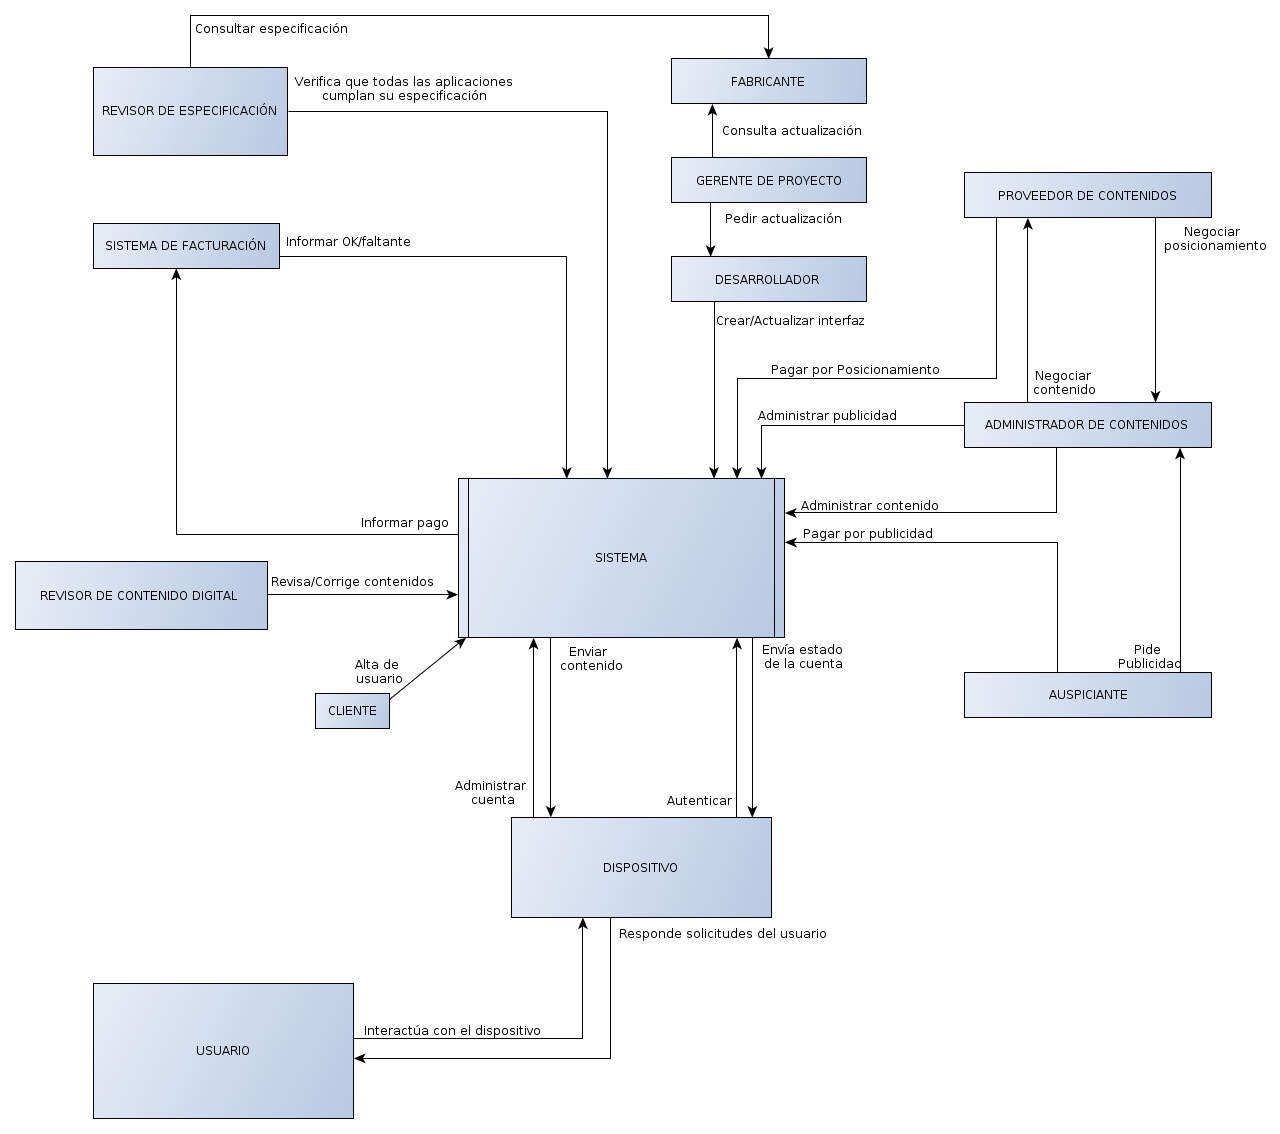
\includegraphics[scale=0.35]{Diagramas/DiagramaContexto.png}
	\end{center}
\subsubsection{Explicaci\'on de agentes e inteacciones no triviales}

\begin{itemize}

\item  {El agente ``sistema`` Es el conjunto de componentes de software y hardware que pertenecen a CentralMarket, una empresa que comercializa contenidos digitales.}

El Sistema se relaciona con varios agentes tanto directa como indirectamente. Ellos son:

\item El agente ``Cliente`` es la persona f\'isica, que registra una cuenta en el sistema. Luego, todas las operaciones que el cliente quiera realizar en el sistema ser\'an referidas como operaciones realizadas por el usuario (la cuenta del cliente).

\item El agente ``Usuario``: es la cuenta desde la cual el cliente se conecta al sistema. El usuario interact\'ua con el sistema pudiendo autenticarse y Administrar su cuenta

\item El agente ``Cliente`` es la persona f\'isica, que registra una cuenta en el sistema. Luego, todas las operaciones que el cliente quiera realizar en el sistema ser\'an referidas como operaciones realizadas por el usuario (la cuenta del cliente).

\item El agente ``Dispositivo``: es una denominaci\'on gen\'erica para referirse al Smart TV, conversor para el televisor anal\'ogico, la computadora, la tablet o al mobile. 

\item La interacci\'on ``Administrar cuenta`` entre el dispositivo y el sistema engloba las siguientes acciones: Comprar contenido, prestar contenido y pedir contenido


\item La interacci\'on ``Responde a las solicitudes del usuario`` entre el dispositivo y el usuario es cuando el dispositivo interpreta los datos que el sistema le env\'ia en respuesta a los pedidos del usuario y los muestra en pantalla.	 
   
\item El agente ``Administrador de contenidos``: es el encargado de conseguir, categorizar, agrupar y posicionar el contenido. Se encarga de asignar publicidad a los contenidos. Tambi\'en es qui\'en decide qu\'ie contenidos pueden prestarse y durante cu\'anto tiempo.

\item El agente ``Auspiciante``: Es la empresa que paga para tener un espacio publicitario en los contenidos que ofrece el sistema.
\item La interacci\'on ``Pide publicidad`` entre los agentes ``Auspiciante y ``Administador de Contenidos`` es cuando el Auspiciante acuerda con el Administrador de contenidos para comprar un espacio publicitario.
  
\item El agente ``Proveedor de Contenidos`` Es la representaci\'on de quienes producen (y en la mayor\'ia de los casos venden) contenido digital. Por ejemplo, Cadenas de Cine, Cadenas televisivas, Productoras musicales, F\'abricas de Software, Editoriales, etc. 

\item La interacci\'on ``Negociar contenido`` entre los agentes ``Administrador de Contenido`` y ``Proveedor de Contenido`` se da cuando el Administrador de Contenidos quiere adquirir cierto contenido de la propiedad del Proovedor de Contenidos. Es el proceso donde se fijan precios y forma de acceso al contenido.
   
\item La interacci\'on ``Negociar posicionamiento`` entre los agente ``Proveedor de Contenido`` sucede cuando el proveedor de contenidos desea que su producto sea desctacado en las b\'usquedas del sistema. Es el proceso donde se fijan los precios y detalles del posicionamiento.

\item El agente ``Revisor de Contenido``: Es el agente que se encarga de revisar y testear los contenidos.

\item El agente ``Revisor de Especificaci\'on``: Es quien debe revisar que los contenidos de ejecuci\'on cumplan la pre y post condici\'on de la especificaci\'on de dichos contenidos.
La especificaci\'on la obtiene del fabricante.

\item El agente ``Fabricante``: Es la representaci\'on de quienes producen software o hardware que se tiene relaci\'on con el sistema. En caso del hardware son los fabricantes de los dispositivos a los que se brinda soporte para utilizar el sistema. En caso de software son los fabricantes de las aplicaciones que se comercializan a trav\'es CentralMarket.

\item El agente ``Gerente de Proyecto``: Es quien se encarga de tomar las decisiones implementativas. Es qui\'en decide cuando hay que actualizar la interfaz de usuario del sistema.

\item El agente ``Desarrollador``: Es qui\'en efectivamente desarrolla y actualiza la interfaz de usuario del sistema.

\item El agente ``Sistema de Facturaci\'on``: es el encargado de registrar los pagos hechos por los clientes, los auspiciantes y los proveedores de contenidos



\end{itemize}

	
\section{Objetivos del sistema}

\subsection{Aclaraciones previas}

	A continuaci\'on describiremos el \emph{Modelo de Objetivos} que proponemos para cumplir los objetivos detallados anteriormente.

	El modelo se conforma por un arbol de objetivos y subobjetivos asociados, c\'omo dicho arbol es extremadamente grande se encuentra 
	dividido en varias partes. Por las reglas del modelo cada hoja del diagrama debe estar asociada a un \emph{agente}, en los casos en que
	una hoja no tenga un agente asociado tendr\'a un n\'umero que corresponde a otro gr\'afico donde el diagrama contin\'ua.
	
\subsection{Objetivos blandos}

	Nuestro sistema se 

	\begin{itemize}

	\item{ Mayor velocidad en contenidos populares: Existen m\'etodos de transferencia de informaci\'on m\'as veloces si los datos a transmitir se 	
	encuentran en una mayor cantidad de m\'aquinas al mismo tiempo. La cantidad de personas que posee un contenido es directamente proporcional a su 
	popularidad.}

	\item{ Mayor estabilidad de velocidad: Sopesa la continuidad en la cantidad de bytes descargados en el tiempo versus r\'afagas quiz\'as m\'as 
	r\'apidas pero no continuas.}

	\item{ Menor costo de implementaci\'on: Este objetivo blando sirve para ver que ramas minimizan el gasto en dinero y tiempo de desarrollo 	
	para poner el sistema en funcionamiento. }

	\item{ Robustez: Intenta responder qu\'e sistema posee los mejores mecanismos para la recuperaci\'on ante fallas.}
    
	\item{ Accesibilidad al contenido: Sirve como eje para el an\'alisis de qu\'e sistema posee m\'as o mejores opciones para acceder al contenido.}

	\item{ Minimizar costos de infraestructura: Sirve para saber cu\'al es el sistema que cumple que minimiza (entre las opciones disponibles) el 
	costo de mantenimiento a lo largo del tiempo.}

	\item{ Proveer contenido de forma m\'as eficiente posible: Es un objetivo blando menos espec\'ifico que los dem\'as, se refiere al equilibrio entre 
	costo computacional, velocidad de respuesta ante pedido, robustez del sistema ante fallas en los canales de comunicaci\'on externos.}

	\end{itemize}

\subsection{Modelo de Objetivos}

	\begin{center}
		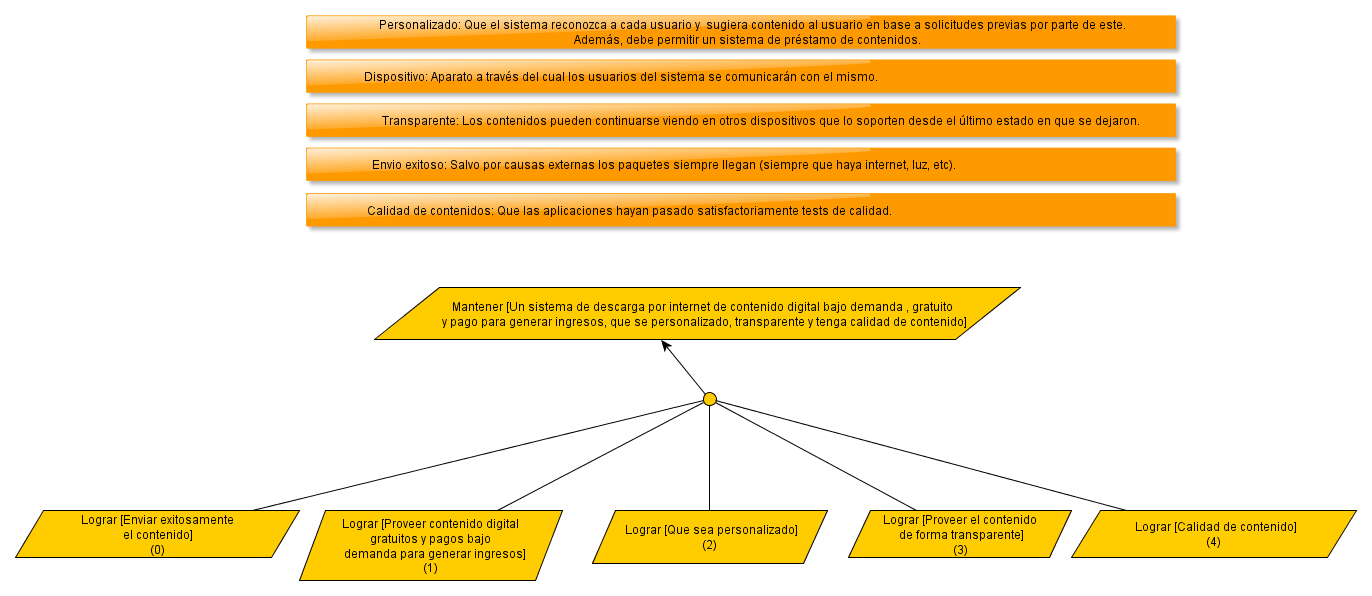
\includegraphics[scale=0.35]{Diagramas/ModelodeObjetivosPrincipal.png}
		\small{Figura Principal: Modelo Principal de Objetivos.}
	\end{center}

\newpage
	\begin{center}
		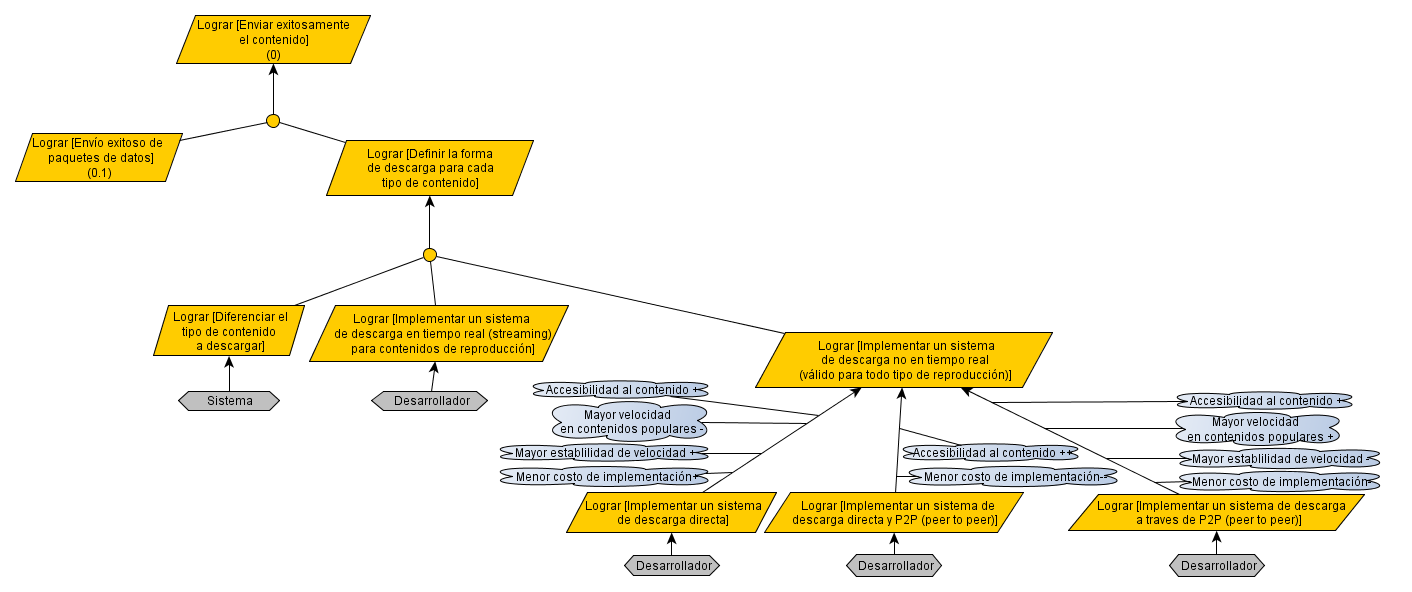
\includegraphics[scale=0.48, angle=90]{Diagramas/0ModelodeObjetivosLograrenviarcontenido.png}
	\end{center}
	\begin{center}
		\small{Figura 0: Env\'io de contenido}
	\end{center}


	Para el env\'io de contenido, se plantea como m\'etodo principal para transmisi'on de contenidos de reproducci\'on utilizar streaming. Adem\'as se agrega un sistema de descarga para todo tipo de contenido, sin necesidad que pueda reproducirse en tiempo real. Para esto se plantean tres opciones distintas, o-refinamientos. Cada uno de ellos posee puntos a favor y en contra que pasan a detallarse a continuaci\'on:
		\begin{itemize}
		\item {Tener un sistema de descarga directa: S\'olo un componente del sistema se encargar\'a del env\'io del contenido, adem\'as el contenido se encuentra en un s\'olo lugar. Como ventajas podemos nombrar que esta forma de implementar la descarga es la m\'as simples de todas y provee una buena estabilidad de velocidad, es decir, como el contenido se encuentra en un lugar s\'olamente, la velocidad de descarga depende \'unicamente de la velocidad del canal de comunicaci\'on entre el sistema y el dispositivo del usuario. La estabilidad en la velocidad aporta negativamente a que los contenidos populares se puedan descargar de manera mas r\'apida. Ayuda adem\'as a la accesibilidad de contenido, ya que los contenidos de reproducci\'on se pueden ver tanto en streaming como de manera posterior a una descarga.}
		\item {Tener un sistema de descarga peer to peer: Utilizar un sistema de descarga peer to peer  posee como ventajas que a mayor cantidad de nodos en una red que contengan el archivo, o partes de \'el, la velocidad de transferencia aumenta. Adem\'as ayuda a la accesibilidad de contenido al igual que el sistema de descarga directa. Como contrapartida una implementaci\'on de un sistema de esta forma es mas complejo, por lo cual su costo aumenta. No se puede asegurar fuertemente la estabilidad de velocidad, ya que esta depende de la velocidad de conexi\'on de todos los dispositivos que est\'en formando parte de la transferencia del archivo.}
		\item {Tener un sistema de descarga directa y peer to peer: Es el sistema m\'as completo de los tres, posee la funcionalidad de elegir descarga directa o descargarlo por peer to peer. Tiene como aporte positivo que supera en accesibilidad a las otras opciones, ya que permite varias formas de descarga para todo los tipos de contenido. Esta funcionalidad extendida provoca como contraparte que aumenta en gran medida el costo de implementaci\'on, siendo el m\'as costoso de las tres opciones en materia de tiempo y dinero invertido.}
		\end{itemize}

\newpage
	\begin{center}
		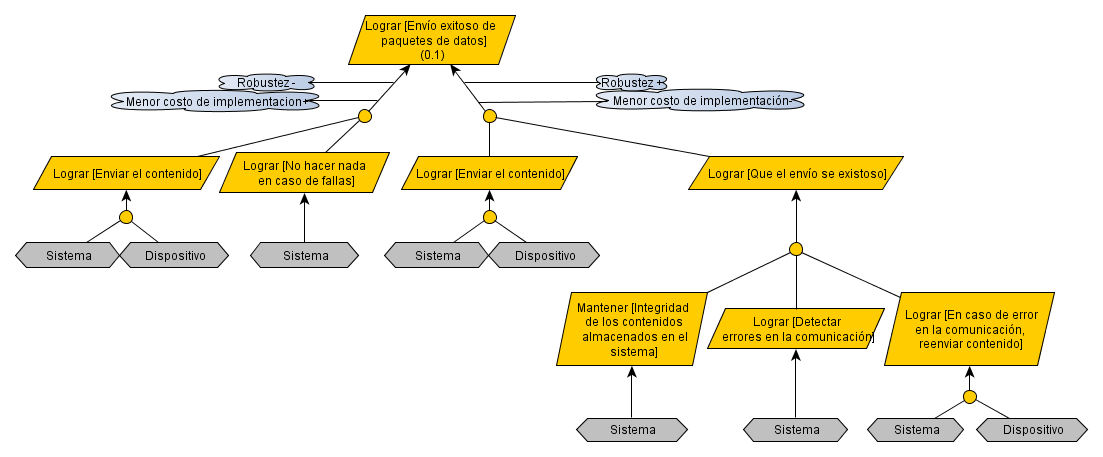
\includegraphics[scale=0.60, angle=90]{Diagramas/0-1ModelodeObjetivosEnvioexitoso.png}
	\end{center}
	\begin{center}
		\small{Figura 1: Env\'io existoso}
	\end{center}
	Se plantean dos opciones para el env\'io de datos de manera exitosa ante la red, el primero de ellos es el m\'as econ\'omico, fallando en su robustez: realizar el env\'io y no hacer nada ante los errores. La segunda opci\'on en cambio si bien es mas costosa plantea un mecanismo de detecci\'on y recuperaci\'on de errores. La robustez del sistema es un sin\'onimo de calidad. Deber\'ia validarse cual es la relaci\'on entre costo implementativo y ganancia en el tiempo por tener un sistema m\'as estable.

\newpage
	\begin{center}
		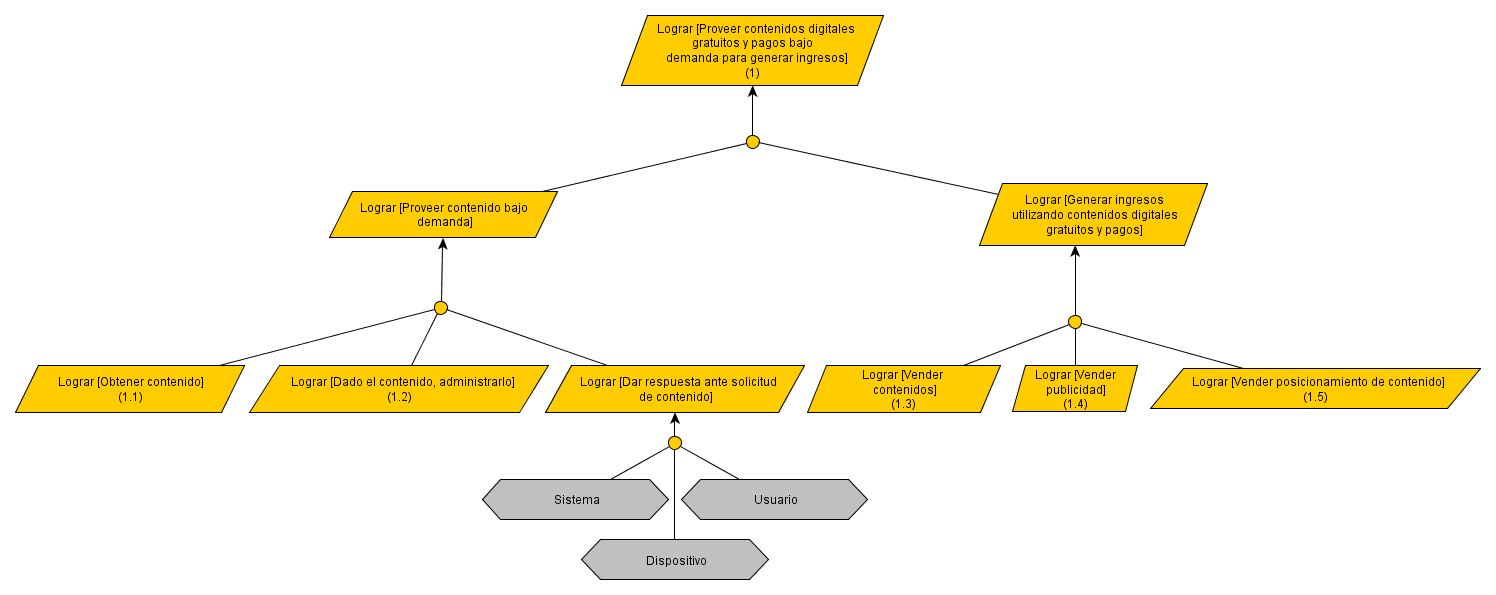
\includegraphics[scale=0.45, angle=90]{Diagramas/1ModelodeObjetivosGenerarIngresos.png}
	\end{center}
	\begin{center}
		\small{Figura 2: Generar ingresos}
	\end{center}
\newpage
	\begin{center}
		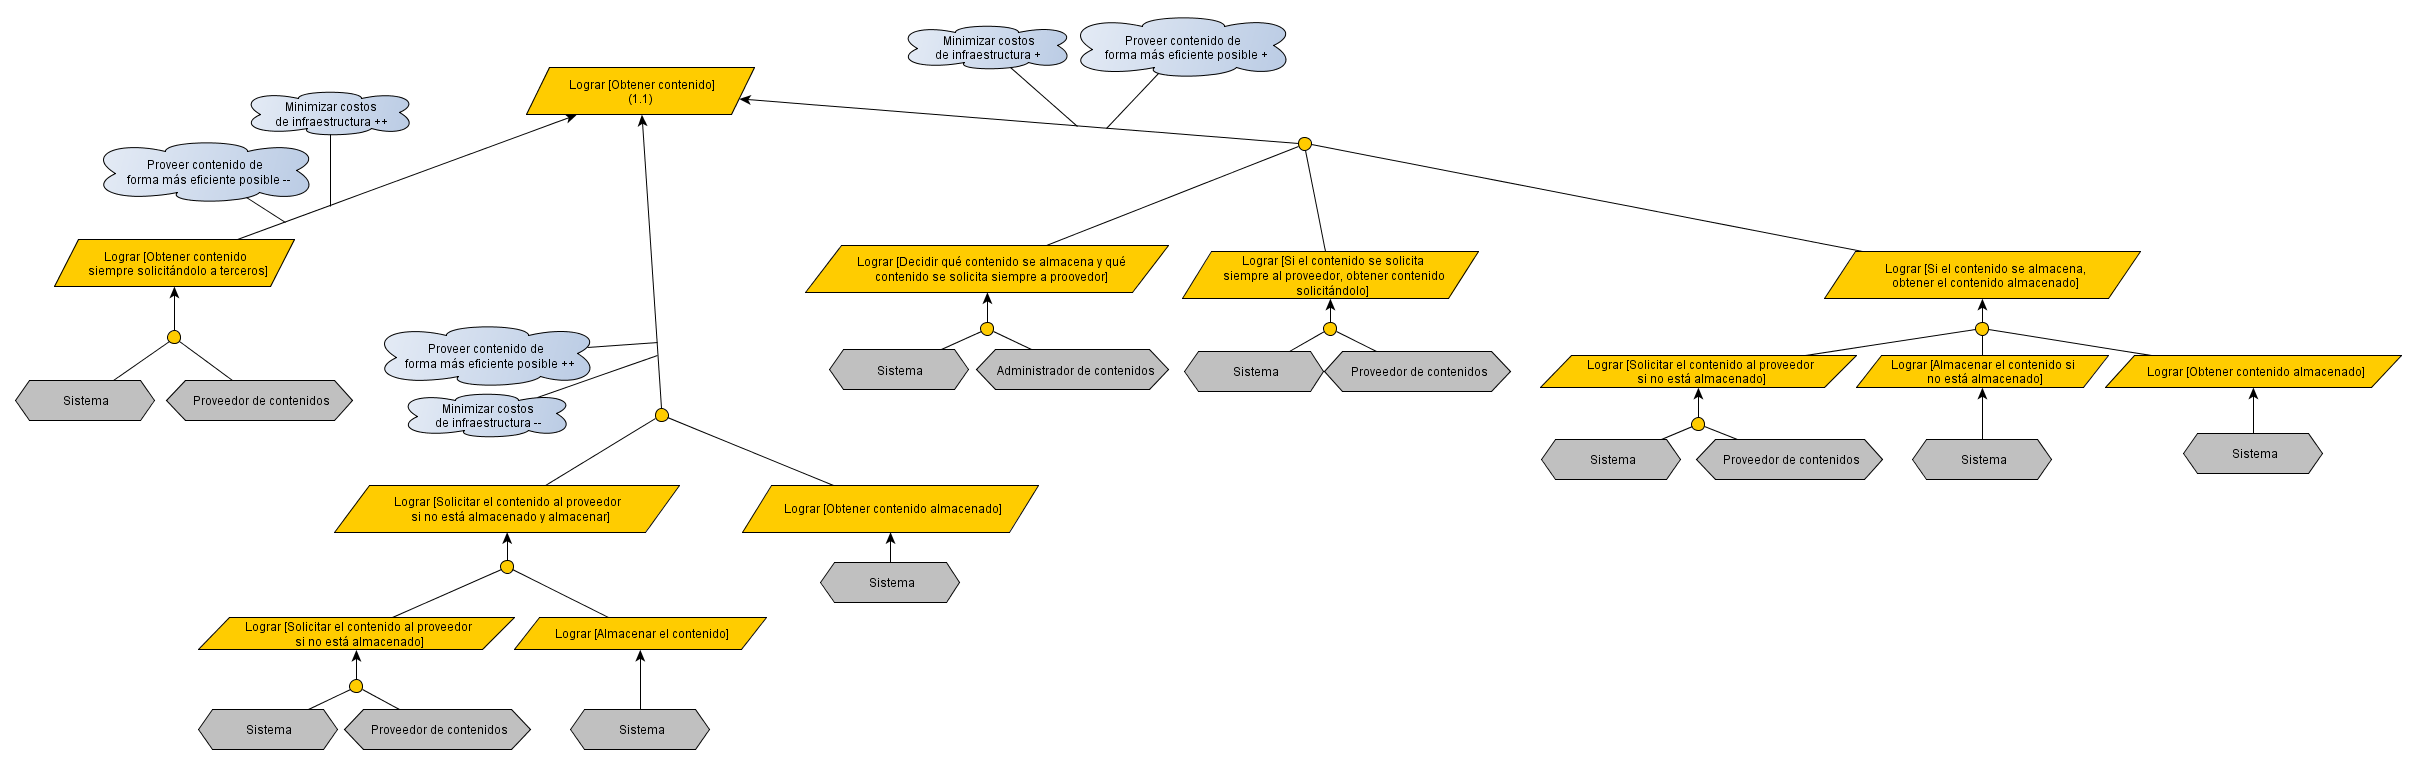
\includegraphics[scale=0.28, angle=90]{Diagramas/1-1ModelodeObjetivosObtenercontenido.png}
	\end{center}
	\begin{center}
		\small{Figura 3: Obtenci\'on de contenido}
	\end{center}

	Se plantean tres formas de obtener contenido: utilizando al sistema de CentralMarket como un nexo entre el proveedor de contenido y el usuario; almacenando todos los contenidos en el sistema de CentralMarket o creando un h\'ibrido entre las dos opciones.

	La primera opci\'on posee a favor que minimiza los costos de infraestructura ya que no se necesita tener grandes vol\'umenes de informaci\'on almacenados en estructuras internas a CentralMarket. Tercerizar el almacenamiento de informaci\'on trae como contrapartida que el canal de comunicaci\'on entre el/los proveedor/es se vuelve cr\'itico, una falla del lado del proveedor/es dejar\'ia a CentralMarket sin sistema y adem\'as la velocidad de respuesta a los usuarios depende en gran medida de la carga que tenga el proveedor y la velocidad de su sistema. 

	El sistema donde toda la informaci\'on se almacena dentro de \'el posee las caracter\'isticas inversas al anterior mencionado. Se encuentran m\'as controlados los posible errores y la velocidad de respuesta teniendo como contrapartida que la inversi\'on y mantenimiento de esta estructura son mayores. 

	El sistema h\'ibrido propone obtener el equilibro entre los dos sistemas antes mencionados, intentar minimizar el costo de mantenimiento en infraestructura manteniendo en la mayor\'ia de contenidos cr\'iticos o importantes una respuesta r\'apida y estable ante los pedidos del usuario.

\newpage
	\begin{center}
		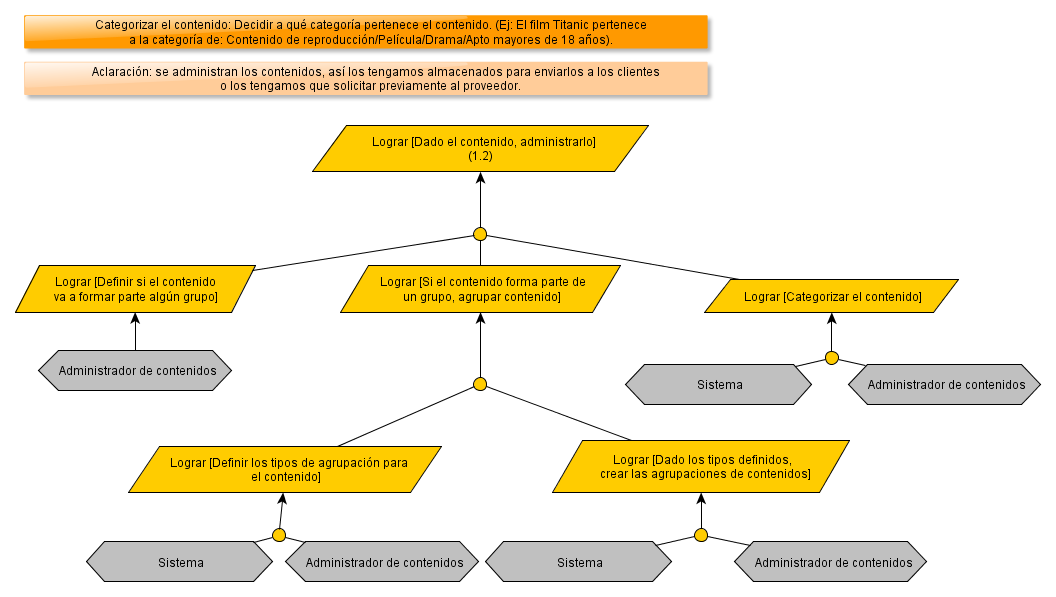
\includegraphics[scale=0.64, angle=90]{Diagramas/1-2ModelodeObjetivosAdministrarcontenido.png}
	\end{center}
	\begin{center}
		\small{Figura 4: Administraci\'on de contenido}
	\end{center}
\newpage
	\begin{center}
		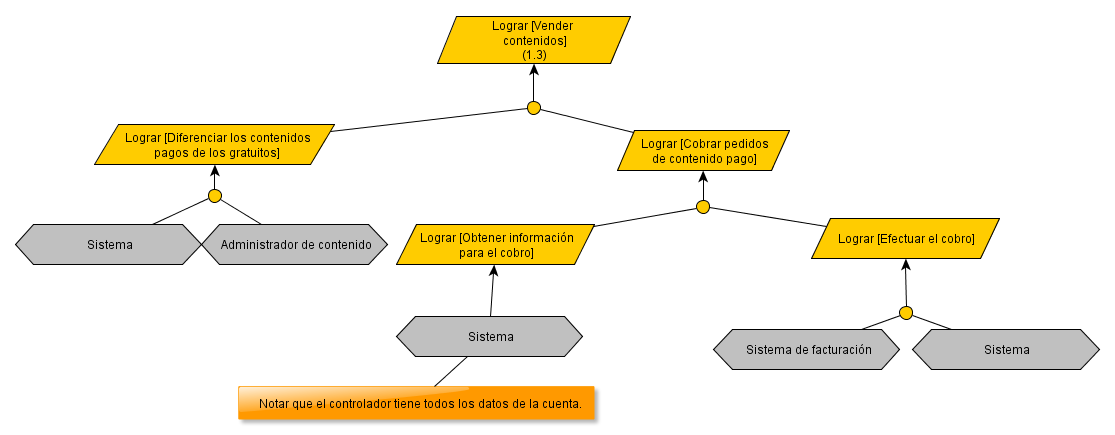
\includegraphics[scale=0.60, angle=90]{Diagramas/1-3ModelodeObjetivosVendercontenido.png}
	\end{center}
	\begin{center}
		\small{Figura 5: Venta de contenido}
	\end{center}
\newpage
	\begin{center}
		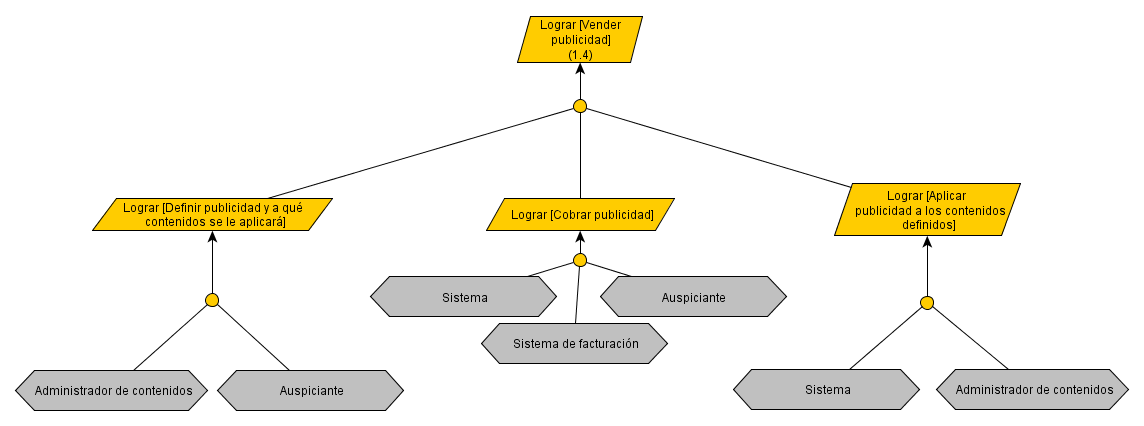
\includegraphics[scale=0.59, angle=90]{Diagramas/1-4ModelodeObjetivosVenderpublicidad.png}
	\end{center}
	\begin{center}
		\small{Figura 6: Venta de publicidad}
	\end{center}
\newpage
	\begin{center}
		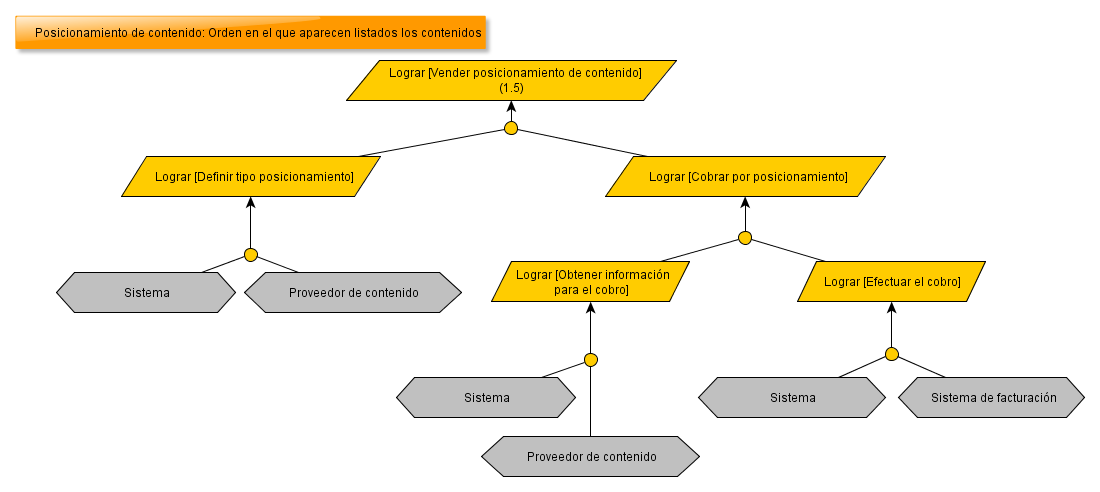
\includegraphics[scale=0.61, angle=90]{Diagramas/1-5ModelodeObjetivosVenderposicionamiento.png}
	\end{center}
	\begin{center}
		\small{Figura 7: Venta de posicionamiento}
	\end{center}
\newpage
	\begin{center}
		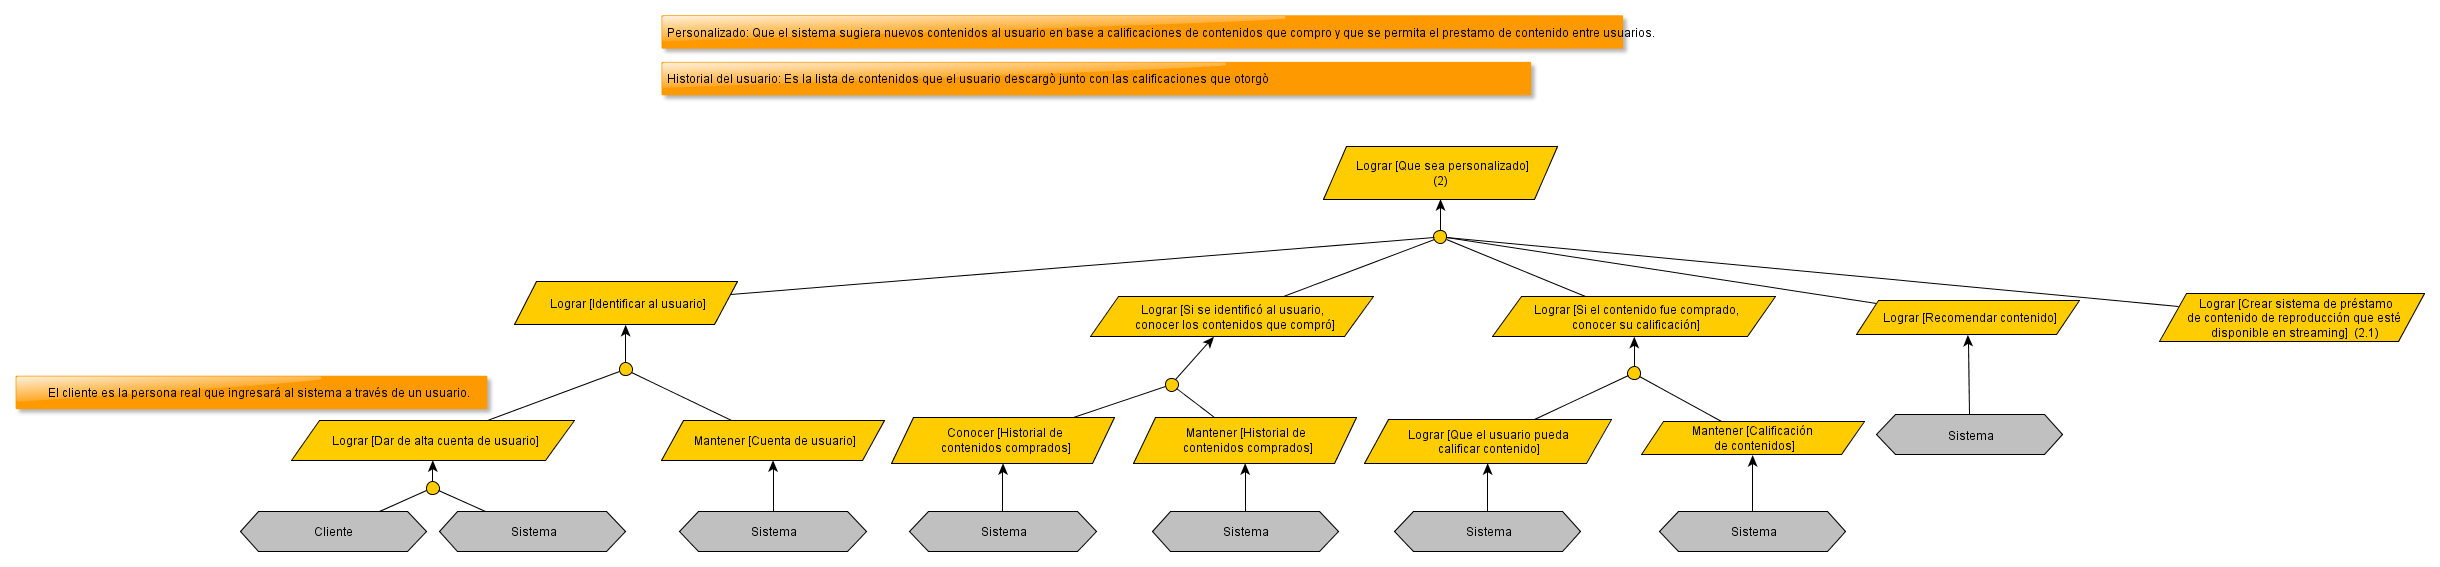
\includegraphics[scale=0.27, angle=90]{Diagramas/2ModelodeObjetivosPersonalizado.png}
	\end{center}
	\begin{center}
		\small{Figura 8: Personalizaci\'on}
	\end{center}
\newpage
	\begin{center}
		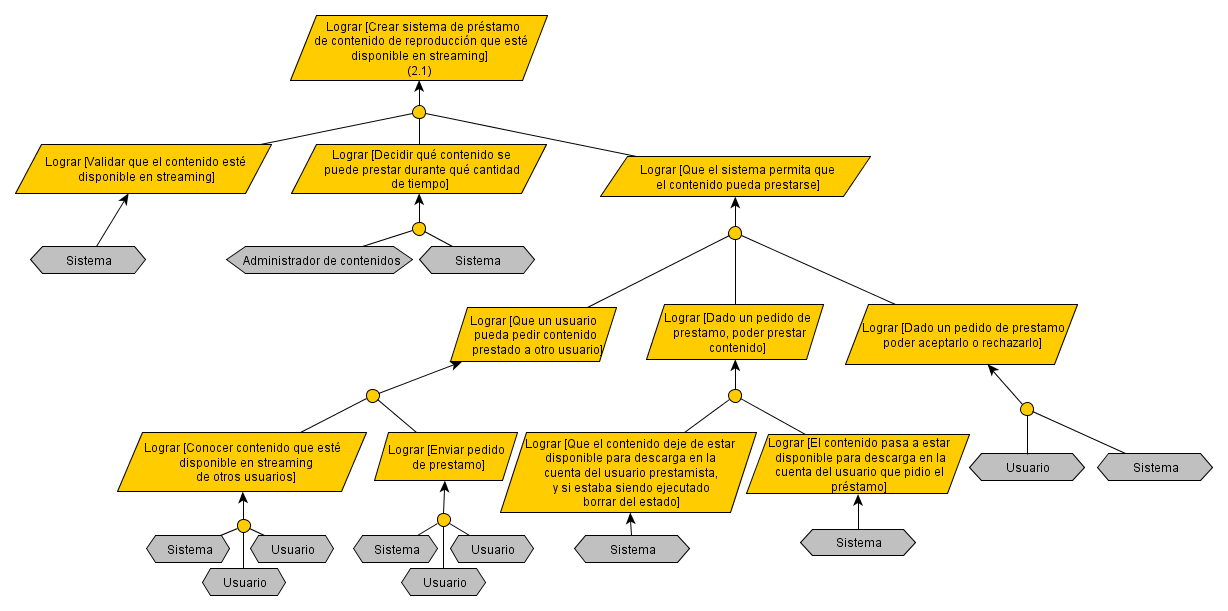
\includegraphics[scale=0.55, angle=90]{Diagramas/2-1ModelodeObjetivosPrestamocontenidos.png}
	\end{center}
	\begin{center}
		\small{Figura 9: Prestamo de contenidos}
	\end{center}
\newpage
	\begin{center}
		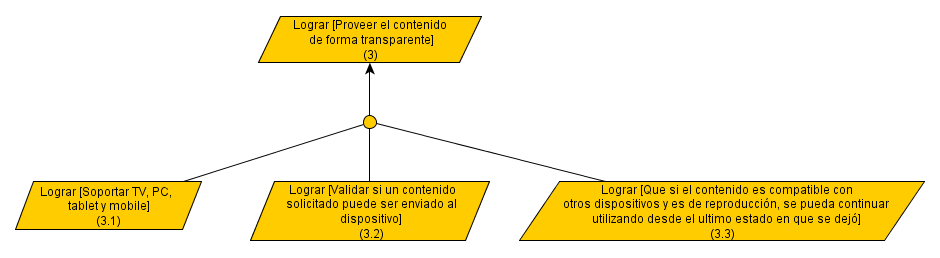
\includegraphics[scale=0.65, angle=90]{Diagramas/3ModelodeObjetivosTransparente.png}
	\end{center}
	\begin{center}
		\small{Figura 10: Transparencia}
	\end{center}
\newpage
	\begin{center}
		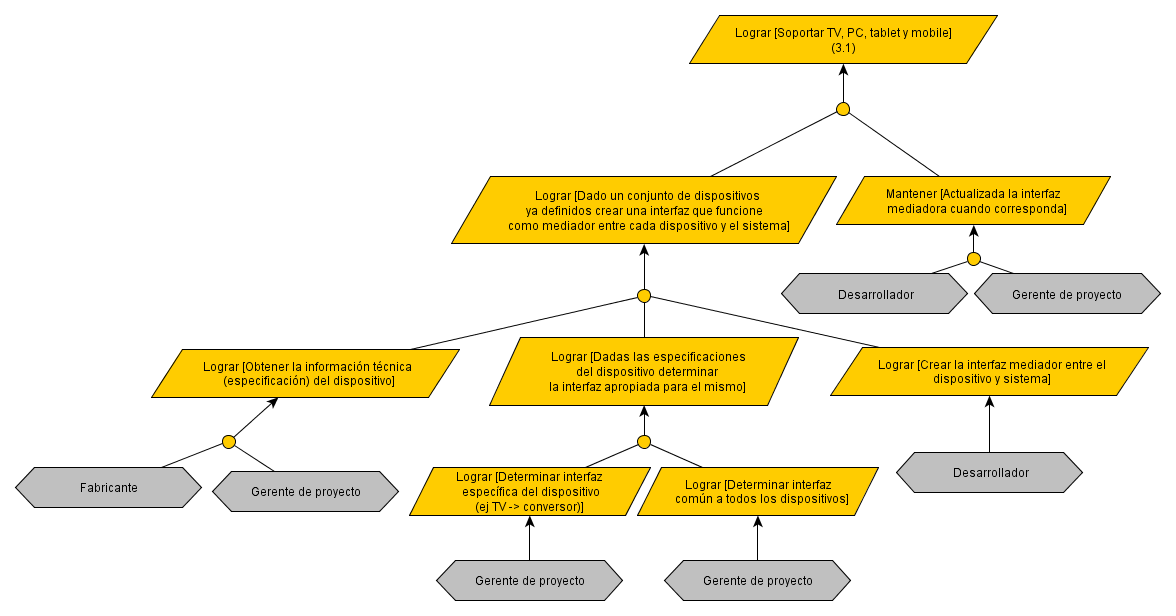
\includegraphics[scale=0.57, angle=90]{Diagramas/3-1ModelodeObjetivosTransparencia.png}
	\end{center}
	\begin{center}
		\small{Figura 11: Transparencia parte 1}
	\end{center}
\newpage
	\begin{center}
		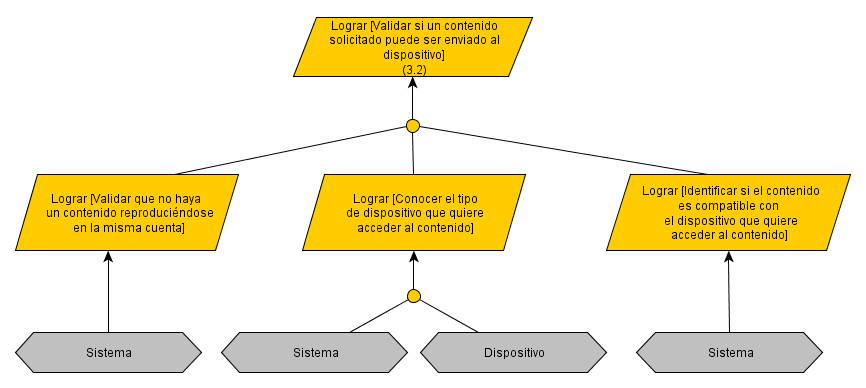
\includegraphics[scale=0.65, angle=90]{Diagramas/3-2ModelodeObjetivosTransparencia.png}
	\end{center}
	\begin{center}
		\small{Figura 12: Transparencia parte 2}
	\end{center}
\newpage
	\begin{center}
		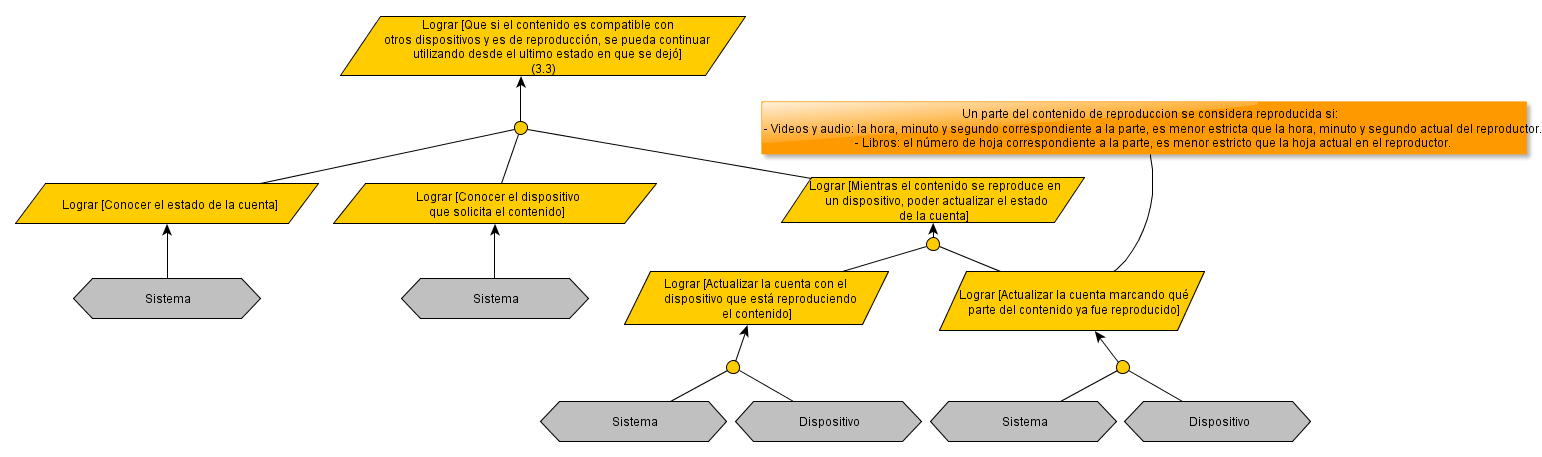
\includegraphics[scale=0.43, angle=90]{Diagramas/3-3ModelodeObjetivosTransparencia.png}
	\end{center}
	\begin{center}
		\small{Figura 13: Transparencia parte 3}
	\end{center}
\newpage
	\begin{center}
		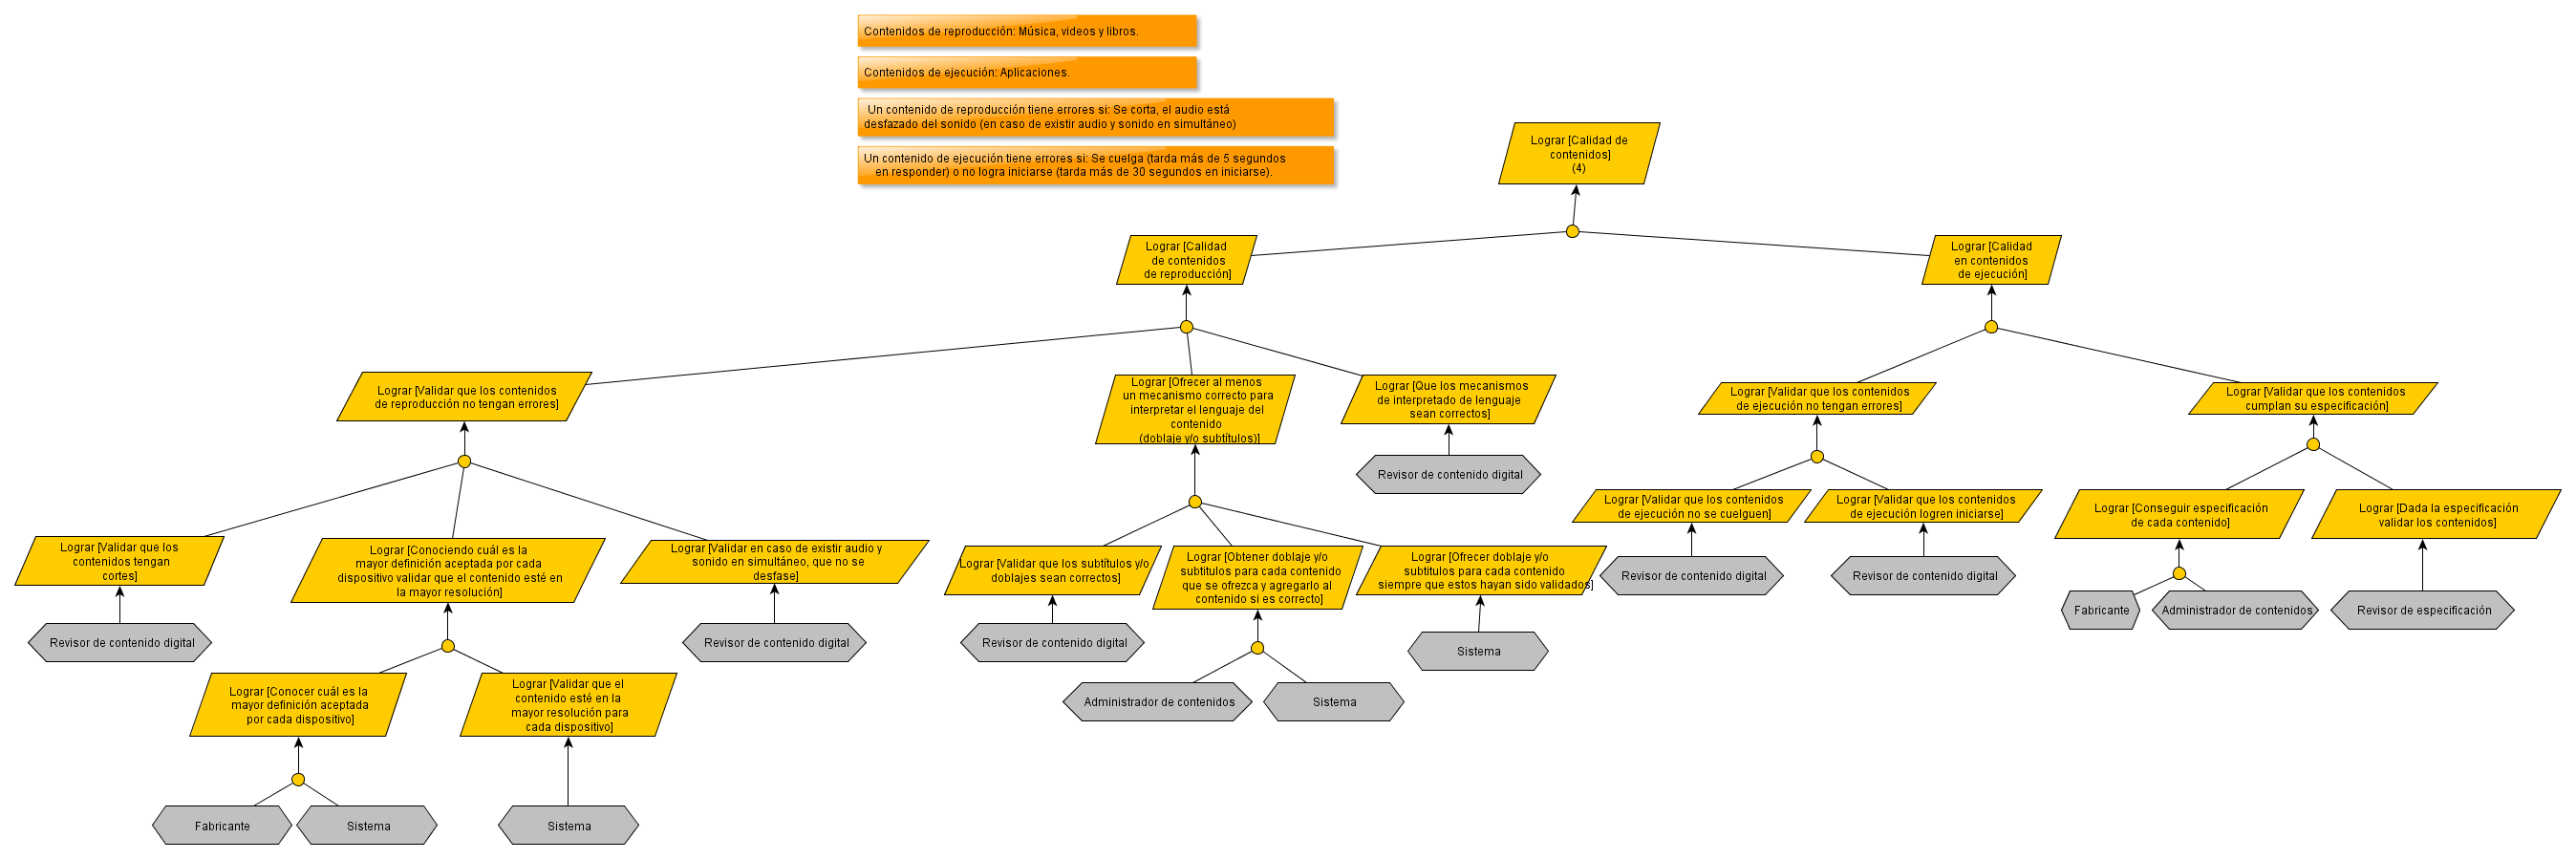
\includegraphics[scale=0.25, angle=90]{Diagramas/4ModelodeObjetivosCalidaddecontenidos.png}
	\end{center}
	\begin{center}
		\small{Figura 14: Calidad de contenidos}
	\end{center}
\newpage


\section{Asunciones}

	Dentro del sistema una cuenta de usuario no puede reproducir m\'as de un contenido por cuenta.
	Si se intenta reproducir otro contenido desde la misma cuenta el sistema no permitir\'a que se haga. 

	El sistema solo permite que los pr\'estamos de libros solo se otorguen por un m\'aximo de 8 semanas.

\newpage

\section{Escenarios informales y ejemplos}
	
	A continuaci\'on se describen una serie de casos que ejemplifican situaciones de funcionamiento esperado del sistema.

\subsection{Situaci\'on 1}

	\textbf{Funcionalidad:} Registro de usuario y baja de un contenido.\\

        Una persona se sienta en frente de la computadora.
    La persona se registra en el sistema (ingresa en la p\'agina del sitio, o descarga 
    la aplicaci\'on dependiendo de la implementaci\'on  de la interfaz de usuario).
    El sistema crea una cuenta y la asocia a esa persona (cliente). As\'i se crea el usuario.
    El usuario busca bajo la categor\'ia de deportes los partidos de f\'utbol locales.
    Encuentra el partido que buscaba (Chacarita vs Atlanta) y comienza a verlo desde su computadora (en streaming).\\

        En el entretiempo, se da cuenta que tiene que cocinar y no quiere dejar de ver el partido. Decide entonces loguearse al sistema desde su 
    tel\'efono inteligente (desde la p\'agina web del sitio o descargando la aplicaci\'on que corresponda). 
    Al autenticarse, la cuenta la cual posee el estado de reproducci\'on, le ofrece continuar viendo el partido desde el instante donde lo dej\'o.
    El cliente acepta y puede llegar a ver como Chacarita mete el segundo gol desde su cocina.

\subsection{Situaci\'on 2}

	\textbf{Funcionalidad:} Publicidad en contenidos.\\

        Un empresario de Powerthrist S.A. (bebida energ\'etica) desea publicitarse y se comunica con el administrador de contenidos de CentralMarket 
    envi\'andole el contenido a publicitar.
    El administrador de contenido le pasa el presupuesto junto con la lista de contenidos que pueden tener la publicidad.
    El empresario acepta y paga con v\'ia online (interactuando con el sistema) quien hace de intermediario con el sistema de facturaci\'on externo.
    El administrador de contenidos aplica entonces la publicidad sobre los contenidos acordados.
    Luego, los usuarios de CentralMarket que adquieran dichos contenidos se encuentran ahora con la publicidad de Powerthrist.

\subsection{Situaci\'on 3}

	\textbf{Funcionalidad:} Compra fallida y exitosa.\\

        Un usuario decide comprar la promoci\'on de verano de pel\'iculas de acci\'on (suponiendo que el gerente de CentralMarket ha dedicido agrupar el     
    contenido de esa forma). Efect\'ua el pago seleccionando de su cuenta una de sus tarjetas registradas. El sistema se comunica con el sistema de 
    facturaci\'on envi\'ando los datos del pago y recibe como respuesta que la tarjeta del usuario no tiene fondos. El sistema comunica al usuario el 
    resultado de la operaci\'on y se cancela la compra de la promoci\'on. El usuario recibe el mensaje y opta por elegir otra tarjeta y reintentar. Esta 
    vez la transacci\'on es exitosa y por consiguiente disfruta del contenido de la promoci\'on durante toda la temporada de verano.

\subsection{Situaci\'on 4}

	\textbf{Funcionalidad:} Obtenci\'on de contenidos y subt\'itulos y validaci\'on de los mismos.\\

        El administrador de contenidos conoce que ya se film\'o la nueva temporada de \emph{The Big Bang Theory}. Por lo tanto se comunica con el 
   proveedor de contenidos quien se los suministra. El administrador le pide adem\'as los subt\'itulos en espa\~{n}ol ya que la mayor\'ia de los subcriptores del 
   sistema son argentinos.

        Como debe cumplir los est\'andares de calidad de CentralMarket, una vez que el contenido ingresa al sistema este debe ser testeado por el revisor 
   de contenido digital previo a lanzamiento al p\'ublico. Es por ello que el revisor ve todos los cap\'itulos de la nueva temporada a publicar y valida 
   que ninguno de ellos se corte, adem\'as, tampoco nota ning\'un desfasaje entre la imagen y sonido. Nota que existen errores en el subt\'itulos por lo 
   tanto, el nuevo contenido todav\'ia no se puede proporcionar al p\'ublico.
   
      El administrador de contenidos vuelve a hablar con el proveedor, quien ahora le suministra unos nuevos subt\'itulos. Estos son vueltos a testear 
   con los cap\'itulos por el revisor quien finalmente los aprueba.

      De esta manera, la nueva temporada de la serie pasa a estar en el sistema como contenido a poder visualizarse. El administrador decide si va a    
   formar parte de un grupo, ser pago o gratuito y finalmente lo agrega al sistema.
   Los usuarios entonces pueden acceder a la reproducci\'on de la nueva serie aclamada de televisi\'on.

\subsection{Situaci\'on 5}

	\textbf{Funcionalidad:} Reproducci\'on de un mismo contenido de la misma cuenta desde dos dispositivos diferentes.\\

      Un usuario decide escuchar m\'usica v\'ia streaming desde su smartphone. El disco que decide escuchar es gratuito. Comienza a reproducirlo y su hija 
   se loguea al sistema con el mismo usuario desde su computadora de escritorio sin saber que su padre lo estaba utilizando desde su smartphone.\\

      La reproducci\'on no se inicia autom\'aticamente en la computadora y un mensaje aparece preguntando si se desea continuar desde el estado en que se   
   dej\'o (es decir en la canci\'on del disco que el padre est\'a escuchando actualmente). El padre no se entera que su hija se logue\'o.\\

      La hija decide no hacerlo, cancelando y entrando a la lista de contenidos de CentralMarket. Encuentra una serie para ver y clickea sobre ella. Se 
   levanta un cartel que dice ``Actualmente hay un contenido en reproducci\'on/descarga. La operaci\'on que ud. desea hacer no puede ser realizada.`` 	  y se vuelve al listado de contenidos.

\subsection{Situaci\'on 6}

	\textbf{Funcionalidad:} Actualizaci\'on de la interfaz del usuario.\\

	Supongamos que la interfaz de CentralMarket consiste en una aplicaci\'on que se instala en los dispositivos.

	Se confirma que se va a sacar un nuevo Service Pack para el sistema operativo Windows 7. Este Service Pack realiza una modificaci\'on sobre la   
   API de Windows lo que provocar\'ia que todos los usuarios utilizando CentralMarket desde una computadora con Windows 7 no puedan utilizar el servicio 
   de forma correcta.\\

       El gerente de proyecto est\'a al tanto de la situaci\'on, se comunica entonces con el fabricante, en este caso la gente de Microsoft y pide el    
   detalle sobre la nueva interfaz de comunicaci\'on con el SO (detalle de la API modificada). Con esta informaci\'on se encarga de avisarle al 
   desarrollador para poder sacar una nueva versi\'on del sistema de CentralMarket compatible con el release del Service Pack de Windows.

\subsection{Situaci\'on 7}

	\textbf{Funcionalidad:} Pr\'estamo de un libro.\\

	Miguel, un cliente de CentralMarket se entera que su amigo Carlos tambi\'en es cliente de la misma compa\~{n}\'ia. Decide buscar mediante el sistema    
   qu\'e contenido posee Carlos en su cuenta y encuentra que hace m\'as de un a\~{n}o compr\'o ``Vuelta al mundo en 80 d\'ias`` de Julio Verne, el libro que siempre quiso leer pero nunca tuvo oportunidad. Decide ped\'irselo prestado por 8 semanas, lapso que el sistema establece para el pr\'estamo de dicho contenido. \\

        En ese momento, Carlos se encontraba reley\'endolo, pero decide prest\'arselo de todas formas. Unas semanas m\'as tarde, Carlos accede a  CentralMarket con el objeto de continuar leyendo su libro. Una vez que accede, se da cuenta que el libro sigue prestado y debe por lo tanto, esperar a que Carlos se lo devuelva teniendo como l\'imite el plazo fijado por el sistema. 

\subsection{Situaci\'on 8}

	\textbf{Funcionalidad:} Autenticaci\'on err\'onea.\\

	Un cliente de CentralMarket desea loguearse al sistema para descargar juegos. Entra al sitio (o abre la aplicaci\'on, dependiendo de la interfaz 
   utilizada), ingresa su nombre de usuario y pone su contrase\~{n}a. La contrase\~{n}a es incorrecta por lo que el sistema le avisa y lo invita a reintentar. 
   Nuevamente la ingresa incorrectamente y nuevamente es avisado.
   Este procedimiento puede realizado infinitas veces.

\subsection{Situaci\'on 9}

	\textbf{Funcionalidad:} Posicionamiento de contenido.\\

	Uno de los proveedores de contenido de CentralMarket desea publicitar una de sus series , una sitcom llamada ``?`Qui\'en me mand\'o a estudiar    
   computaci\'on?!``, que debido a su poco \'exito no est\'a consiguiendo cubrir los costos de su producci\'on, y para esto se comunica con el administrador de 
   contenido quien le informa que si paga la tarifa adecuada, este puede posicionarla en los primeros lugares cuando los usuarios realicen alguna    
   b\'usqueda en la cual esta sitcom est\'e relacionada. Al aceptar, el proveedor de contenido realiza el pago en el sistema, y espera que las cr\'iticas    
   mejoren para poder vender una nueva temporada de su serie a las cadenas televisivas y otras empresas. 


\subsection{Situaci\'on 10}

	\textbf{Funcionalidad:} Descarga de contenidos y almacenado de los mismos .\\

	Un usuario decide poder acceder a un contenido. Por lo tanto se loguea al sistema, lo busca entre la lista de contenido y lo selecciona, para 
   accederlo. Desde el sistema, se recibe el pedido y lo procesa.\\

       Si se trata de un contenido gratuito, lo obtiene. Si se trata de un contenido pago, el sistema coteja el producto solicitado con el historial de 
   compras del usuario para determinar si debe cobrarle el acceso o no. En caso de que ya lo haya comprado, obtiene el contenido; sino le ofrece la opci
   \'on de compra.\\
   La forma de obtenerlo depender\'a del refinamiento elegido. Puede ser alguna de las siguientes:

	\begin{itemize}
	
	\item{ El sistema recibe el pedido y se se comunica con la interfaz del proveedor que posee ese contenido, requiri\'endoselo. El contenido le 
   llega al sistema que lo re-codifica para ser entendible por el dispositivo del usuario. Dependiendo del tr\'afico de red o carga de procesamiento 
   del proveedor, el sistema, y por consiguiente el usuario, puede llegar a quedarse esperando indefinidamente respuesta.}

	\item{ El sistema recibe el pedido y, si el contenido no est\'a en el sistema, se comunica con la interfaz del proveedor que posee ese 
   contenido almacen\'andolo a medida que realiza el env\'io al usuario para en posteriores pedidos, para ya en un futuro ya tenerlo disponible y no 
   necesitar pedirlo nuevamente al proveedor. Si est\'a almacenado, simplemente comienza la transferencia.}

	\item{ Para minimizar los costos de mantenimiento de infraestructura, el administrador de contenidos decide que (dada la posibilidad que ofrece 
   el sistema de elegir cu\'ando guardar el contenido en servidores propios) se van a almacenar s\'olo los contenidos que se hayan solicitado m\'as de 
   100 veces en el lapso de una semana, quiere as\'i minimizar el tr\'afico de red y economizar espacio.}

	De Lunes a S\'abado recibe 99 pedidos de descarga de un juego de videos para la computadora. En cada uno de estos pedidos, el sistema se 
   comunica con el proveedor pidi\'endole el contenido y d\'andoselo al usuario.

	El d\'ia Domingo recibe el pedido n\'umero 100 y por lo tanto debe esta vez pedirlo al proveedor y a su vez almacenarlo. Resulta ser una buena 
   desici\'on ya que en el correr de la semana siguiente, se realizan cientos de pedidos del mismo juego a CentralMarket y se logra evitar el tr\'afico 
   de red con el proveedor.

	\end{itemize}

\subsection{Situaci\'on 11}

	\textbf{Funcionalidad:} Agregado de una nueva aplicaci\'on al sistema de CentralMarket .\\

	Una nueva aplicaci\'on causa sensaci\'on en internet. Se ve factible que forme parte del paquete de programas de CentralMarket. Este contenido, 
   mediante el administrador de contenidos, se incluye en el sistema para el an\'alisis funcional y test. Como el administrador sabe, un contenido de 
   ejecuci\'on no puede agregarse en el sistema sin que el contenido este excento de errores (no se cuelgue y logre iniciarse) y sin tener una 
   especificaci\'on; luego este no puede distribuirse si no cumple satisfactoriamente la revisi\'on de los mismos.

	El encargado de validar el correcto funcionamiento de la aplicaci\'on entra en juego: el revisor de especificaci\'on. Realiza un exhaustivo 
   an\'alisis de la aplicaci\'on, probando que valgan la pre y post condici\'on, testeando casos bordes y casos esperados sin poder encontrar un 
   comportamiento no esperado.

	Pasa entonces a la segunda etapa, considerada como el test de estr\'es sobre la aplicaci\'on. El revisor de contenido digital es encargado de 
   validar que el contenido no posea errores, es decir que la aplicaci\'on no se cuelgue por mas de cinco segundos y que logre iniciarse en menos de 
   treinta. El testeo es exitoso y pasa a la etapa de an\'alisis funcional.

	Terminado esto, se puede concluir que el programa cumple correctamente la especificaci\'on y est\'a excento de errores, por lo tanto puede ser 
   agregado a la lista de contenidos de ejecuci\'on a distribuir.
        Efectivamente, el programa causa sensaci\'on entre los usuarios de CentralMarket, lo que ayuda m\'as a\'un para generar satisfacci\'on entre los 
   usuarios.

\end{document}
